% Copyright 2023  Ed Bueler

\documentclass[10pt,
               svgnames,
               hyperref={colorlinks,citecolor=DeepPink4,linkcolor=FireBrick,urlcolor=Maroon},
               usepdftitle=false]{beamer}

\mode<presentation>
{
  \usetheme{Madrid}

  \usecolortheme{beaver}

  \setbeamercovered{transparent}
  
  \setbeamerfont{frametitle}{size=\large}
}

\setbeamercolor*{block title}{bg=red!10}
\setbeamercolor*{block body}{bg=red!5}

\usepackage[english]{babel}
\usepackage[latin1]{inputenc}
\usepackage{times}
\usepackage[T1]{fontenc}
% Or whatever. Note that the encoding and the font should match. If T1
% does not look nice, try deleting the line with the fontenc.

\usepackage{empheq,bm,xspace,minted}
\usepackage{hyperref}
\usepackage{tikz}

% If you wish to uncover everything in a step-wise fashion, uncomment
% the following command: 
%\beamerdefaultoverlayspecification{<+->}

\newcommand{\bb}{\mathbf{b}}
\newcommand{\bc}{\mathbf{c}}
\newcommand{\be}{\mathbf{e}}
\newcommand{\bbf}{\mathbf{f}}
\newcommand{\bl}{\bm{\ell}}
\newcommand{\br}{\mathbf{r}}
\newcommand{\bs}{\mathbf{s}}
\newcommand{\bu}{\mathbf{u}}
\newcommand{\bv}{\mathbf{v}}
\newcommand{\bw}{\mathbf{w}}
\newcommand{\bx}{\mathbf{x}}
\newcommand{\by}{\mathbf{y}}
\newcommand{\bz}{\mathbf{z}}

\newcommand{\bzero}{\bm{0}}

\newcommand{\CC}{\mathbb{C}}
\newcommand{\RR}{\mathbb{R}}

\newcommand{\ddt}[1]{\ensuremath{\frac{\partial #1}{\partial t}}}
\newcommand{\ddx}[1]{\ensuremath{\frac{\partial #1}{\partial x}}}
\renewcommand{\t}[1]{\texttt{#1}}
\newcommand{\Matlab}{\textsc{Matlab}\xspace}
\newcommand{\Octave}{\textsc{Octave}\xspace}
\newcommand{\eps}{\epsilon}

\newcommand{\grad}{\nabla}
\newcommand{\Div}{\nabla \cdot}

\newcommand{\ds}{\displaystyle}
\newcommand{\twovect}[4]{\ensuremath{{#1}_{#2} =
                            \begin{bmatrix} #3 \\ #4 \end{bmatrix}}}



\title{Multigrid}

\subtitle{optimal solvers for linear and nonlinear elliptic PDEs}

\author{Ed Bueler}

\institute[]{UAF Math 692 Scalable Seminar}

\date{Spring 2023}


\begin{document}
\beamertemplatenavigationsymbolsempty

\begin{frame}
  \maketitle
\end{frame}

\begin{frame}{Outline}
  \tableofcontents[hideallsubsections]
\end{frame}


\section{examples: two elliptic PDE problems}

\begin{frame}{a linear PDE problem}

\begin{columns}
\begin{column}{0.6\textwidth}
\begin{itemize}
\item I will consider only two PDEs today
    \begin{itemize}
    \item[1.] Poisson problem
    \item[2.] minimal surface problem
    \end{itemize}
\item elliptic boundary-value problems
\item recall Laplacian
    $$\grad^2 u =\Div(\grad u)$$

    \begin{itemize}
    \item[$\circ$] in 2D: \quad $\grad^2 u = u_{xx} + u_{yy}$
    \item[$\circ$] $\grad^2$ is a negative-definite operator
    \end{itemize}
\end{itemize}
\end{column}
\begin{column}{0.4\textwidth}
\hfill 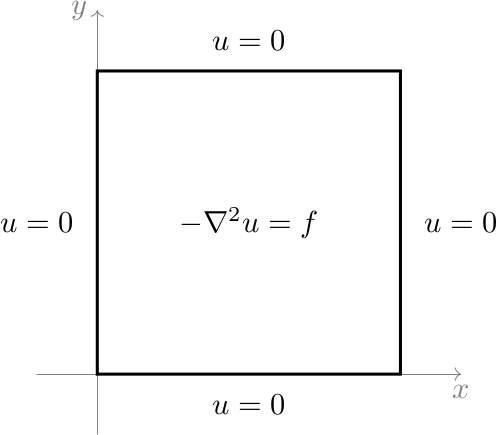
\includegraphics[width=\textwidth]{images/poisson.png}
\end{column}
\end{columns}

\bigskip
\begin{block}{1.~Poisson problem} for a given source function $f(x,y)$, find $u(x,y)$ so that
    $$-\grad^2 u = f \, \text{ on } \Omega, \qquad u\big|_{\partial \Omega} = 0$$
\end{block}
\end{frame}


\begin{frame}{a nonlinear PDE problem}

\begin{columns}
\begin{column}{0.7\textwidth}
\begin{itemize}
\item the second problem is nonlinear, but still elliptic
\item \textbf{claim 1.} the area of surface $z=v(x,y)$ over $\Omega$ is
    $$I[v] = \int_\Omega \sqrt{1 + |\grad v|^2}\,dx\,dy$$
\item \textbf{claim 2.} for given $g$, continuous along $\partial\Omega$,
    $$u = \min_{\{v \,:\, v|_{\partial \Omega} = g\}} I[v]$$
solves the boundary value problem below
\end{itemize}
\end{column}
\begin{column}{0.3\textwidth}
\hfill 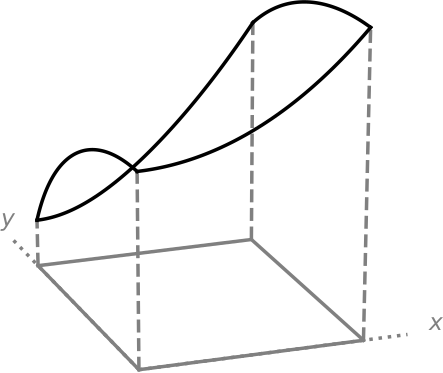
\includegraphics[width=0.75\textwidth]{images/catenary.png}

\hfill 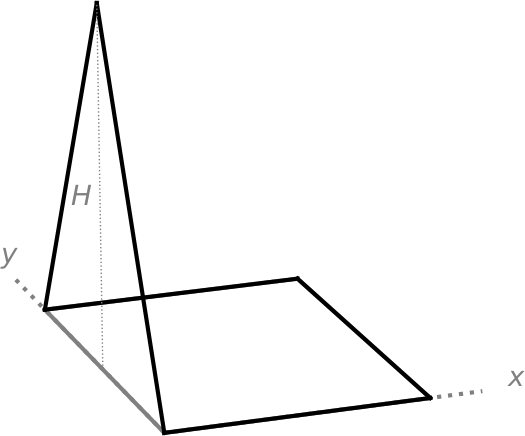
\includegraphics[width=0.75\textwidth]{images/tent.png}
\end{column}
\end{columns}

\medskip
\begin{block}{2.~minimal surface problem} for given boundary function (wire frame) $g(x,y)$, find $u(x,y)$ so that
    $$-\Div \left(\frac{\grad u}{\sqrt{1 + |\grad u|^2}}\right) = 0 \, \text{ on } \Omega, \qquad u\big|_{\partial \Omega} = g$$
\end{block}
\end{frame}


\begin{frame}{finite difference discretization}
\begin{columns}
\begin{column}{0.7\textwidth}
\begin{itemize}
\item PDEs are infinite-dimensional problems, but \textbf{discretization} yields finite systems of equations
\item for example, finite differences (FD):
    $$f''(x) = \frac{f(x+h) - 2 f(x) + f(x-h)}{h^2} + O(h^2)$$
\item assume: $\Omega = (0,1) \times (0,1)$
\item grid spacings: \strut $h_x=\frac{1}{m_x-1}$, $h_y=\frac{1}{m_y-1}$
\item grid points: $(x_i,y_j) = (ih_x,jh_y)$ for $i=0,\dots,m_x-1$ and $j=0,\dots,m_y-1$
\item 5-point stencil for the Laplacian:
{\small
$$\grad^2 u(x_i,y_j) \approx \frac{u_{i-1,j} - 2 u_{ij} + u_{i+1,j}}{h_x^2} + \frac{u_{i,j-1} - 2 u_{ij} + u_{i,j+1}}{h_y^2}$$
}
\end{itemize}
\end{column}
\begin{column}{0.3\textwidth}
\hfill 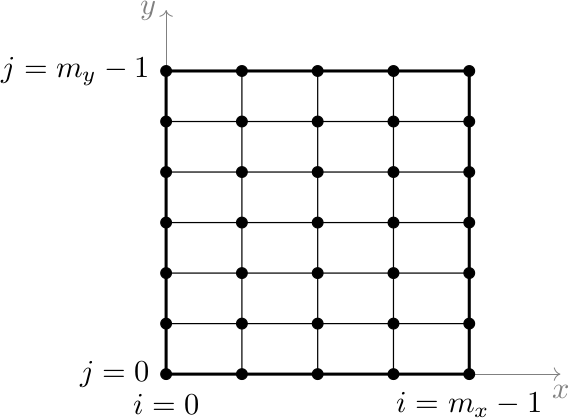
\includegraphics[width=\textwidth]{images/gridindexing.png}

\vspace{15mm}
\hfill 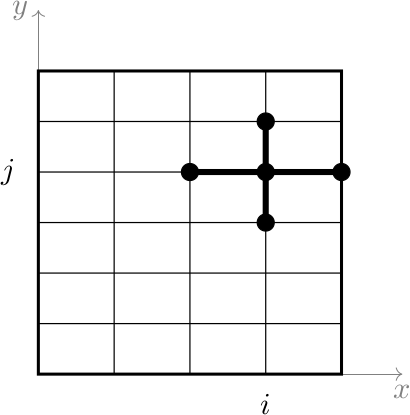
\includegraphics[width=0.7\textwidth]{images/gridstencil.png}
\end{column}
\end{columns}
\end{frame}


% next slide spy plots from Matlab (NOT OCTAVE):
%   m=5; spy(delsq(numgrid('S',m)),'k'), axis off,  print -dpdf lapspy5.pdf
%   m=8; spy(delsq(numgrid('S',m)),8,'k'), axis off,  print -dpdf lapspy8.pdf
% then pdfcrop

\begin{frame}{PDE $\implies$ linear system $A\,\bu=\bb$}
\begin{columns}
\begin{column}{0.73\textwidth}
\begin{itemize}
\item FD discretize $-\grad^2 u = f$

	\begin{itemize}
	\item[$\circ$] $N=m_x m_y$ total unknowns on the grid
	    \begin{itemize}
	    \item $m_x=4,m_y=3$ shown at right
        \end{itemize}
	\item[$\circ$] unknowns $\{u_{ij}\}$ are globally ordered using $k=0,1,\dots,N-1$
	\item[$\circ$] note we keep the boundary values in the system
	\end{itemize}
\item get a linear system for $\bu \in \RR^N$:
	$$A\, \bu = \bb$$

	\begin{itemize}
	\item[$\circ$] $A \in \RR^{N\times N}$ is \textbf{sparse}
	\item[$\circ$] $A$ has positive diagonal
	\item[$\circ$] $A$ is symmetric positive definite
	\item[$\circ$] $\bb \in \RR^N$ has entries $b_k = f(x_i,y_j)$
	\end{itemize}
\item for $m_x=m_y=5$: \,\,\,9 non-trivial eqns (middle right)
\item for $m_x=m_y=8$: 36 non-trivial eqns (lower right)
\end{itemize}
\end{column}
\begin{column}{0.27\textwidth}
\hfill 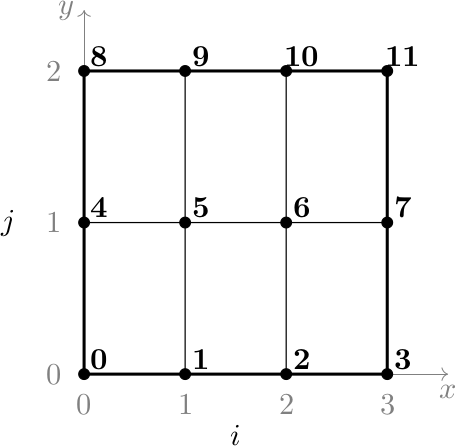
\includegraphics[width=0.9\textwidth]{images/gridordering.png}

\bigskip\medskip
\hfill 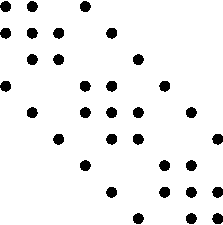
\includegraphics[width=0.5\textwidth]{images/lapspy5.pdf} \hspace{5mm}

\bigskip
\hfill 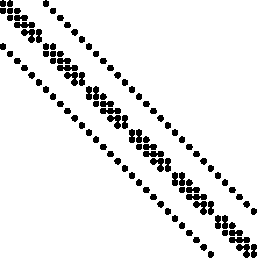
\includegraphics[width=0.7\textwidth]{images/lapspy8.pdf}

\end{column}
\end{columns}
\end{frame}


\begin{frame}{goal: solve $A\,\bu=\bb$ in $O(N)$ work}
\begin{itemize}
\item the linear system $A\,\bu=\bb$ can be set-up using  $6N$ memory locations
	\begin{itemize}
	\item[$\circ$] $A$ has 5 nonzero entries per row, plus one entry of $\bb$
	\end{itemize}
\item how to solve $A\,\bu=\bb$ in $O(N)$ work and time as $N\to\infty$?
	\begin{itemize}
	\item[$\circ$] if so, the solver is \emph{optimal}
	\end{itemize}

\bigskip
\item<2-> $A$ is banded, with bandwidth $\approx \min\{m_x,m_y\} \approx \sqrt{N}$
	\begin{itemize}
	\item[$\circ$] so banded Gaussian elimination will solve in $O(N^2)$
	\end{itemize}

\bigskip
\item<3> let's back up and ask:

\medskip
\qquad what operations using our $A$ are obviously $O(N)$?
\end{itemize}
\end{frame}


\begin{frame}{cheap $O(N)$ operations: mat-vec $A\bv$, and the residual}
\begin{itemize}
\item for $A$ from PDE discretization, we can compute $A\bv$ in $O(N)$ flops
	\begin{itemize}
	\item[$\circ$] this is because $A$ has $O(1)$ nonzero entries per row
	\end{itemize}
\item also the residual is $O(N)$
\end{itemize}

\bigskip
\begin{definition} given $\bv \in\RR^N$, the \emph{residual} for the linear system $A\,\bu=\bb$ is
	$$\br(\bv) = \bb - A\bv$$
observe that:
    $$A\,\bu = \bb \quad \iff \quad \br(\bu) = 0$$
\end{definition}
\end{frame}


\section{simple iterations?}

\begin{frame}{are simple iterations cheap $O(N)$ operations?}

\begin{definition} for the linear system $A\,\bu=\bb$ and an invertible matrix $M\in \RR^{N\times N}$, \emph{simple iteration} is
    $$\bv_{k+1} = \bv_k + \alpha\, M^{-1} \underbrace{\left(\bb - A \bv_k\right)}_{=\,\br(\bv_k)}$$
\end{definition}

\begin{itemize}
\item $\alpha\in\RR$ is a tuning parameter, with default $\alpha=1$
\item if $M=A$ and $\alpha=1$ then $\bv_{k+1}=\bu$, so one iteration solves it!
	\begin{itemize}
	\item[$\circ$] \dots not practical
	\end{itemize}
\item \emph{Richardson iteration} \quad $\bv_{k+1} = \bv_k + \alpha\, \br(\bv_k)$ \quad is the $M=I$ case
	\begin{itemize}
	\item[$\circ$] observation: Richardson iteration for the Poisson equation is \emph{gradient descent} for the quadratic functional \quad $\displaystyle I[v] = \alpha \int_\Omega \frac{1}{2} |\grad v|^2 - f v$
	\item[$\circ$] each Richardson iteration is clearly $O(N)$ work
	\end{itemize}

\medskip
\item a simple iteration is $O(N)$ \dots \emph{if} $M$ is the right kind of matrix!
\end{itemize}
\end{frame}


\begin{frame}{preconditioned linear systems}

\begin{definition} if a matrix or linear map $M \in \RR^{N\times N}$ is invertible, we say
    $$M^{-1} A \bu = M^{-1} \bb$$
is a \emph{(left-) preconditioned} system for $A\,\bu=\bb$
\end{definition}

\begin{itemize}
\item the preconditioned system has the same solutions as before
\item the new residual is \, $\tilde{\br}(\bv) = M^{-1} \bb - M^{-1} A \bv$
\item observation: Richardson iteration on the new system is equivalent to simple iteration
    $$\bv_{k+1} = \bv_k + \alpha\, \tilde{\br}(\bv) \quad \iff \quad \bv_{k+1} = \bv_k + \alpha\, M^{-1} \left(\bb - A \bv_k\right)$$
\end{itemize}
\end{frame}


\begin{frame}{fast preconditioners?}

\begin{definition} a matrix or linear map $M$ is a \emph{fast preconditioner} if solving $M\,\bz=\bc$ requires $O(N)$ work
\end{definition}

\begin{itemize}
\item example: if $A$ has nonzero diagonal entries, the diagonal $M=D$ is a fast preconditioner
\item do \emph{not} actually form the matrix $M^{-1}$ when solving $M\,\bz=\bc$
\item warning: a preconditioner $M$ can be fast without being a useful tool!
\item preconditioning is an apparently simple idea, but in the 21st century it is used all over the space of solvers
\end{itemize}
\end{frame}


\begin{frame}{$O(N)$ simple iterations: Jacobi and Gauss-Seidel}
\begin{itemize}
\item suppose we split $A$ into diagonal and triangular parts:
	$$A=D + L + U$$
\only<1>{
\item the linear system can be rearranged using the splitting:
\begin{align*}
A\,\bu=\bb \quad &\iff \quad D \bu = \bb - (L+U) \bu \\
               &\iff \quad \bu = \bu + D^{-1} (\bb - A \bu)
\end{align*}
\item solving $D\bz = \bc$ is $O(N)$
\begin{definition}
a \emph{Jacobi iteration} applies a fast preconditioner:
	$$\bv_{k+1} = \bv_k + D^{-1} (\bb - A \bv_k)$$
\end{definition}
}
\only<2>{
\item the linear system can be rearranged using the splitting:
\begin{align*}
A\,\bu=\bb \quad &\iff \quad (D+L) \bu = \bb - U \bu \\
               &\iff \quad \bu = \bu + (D+L)^{-1} (\bb - A \bu)
\end{align*}
\item solving $(D+L)\bz=\bc$ is $O(N)$ (for our $A$)

\begin{definition}
a \emph{Gauss-Seidel (GS) iteration} applies a fast preconditioner:
	$$\bv_{k+1} = \bv_k + (D+L)^{-1} (\bb - A \bv_k)$$
\end{definition}
}
\end{itemize}
\end{frame}


\begin{frame}{example of Gauss-Seidel iteration}
\begin{itemize}
\item the matrix-splitting view obscures the simplicity of Gauss-Seidel?
\item \emph{example}: consider the linear system $A\bu=\bb$ with
    $$A = \begin{bmatrix} 2 & -1 & & & & \\ -1 & 2 & -1 & & & \\ & -1 & 2 & -1 & & \\ & & \ddots & \ddots & \ddots & \\ & \Big. & & -1 & 2 & -1 \\ & & & & -1 & 2 \end{bmatrix}, \qquad \bb = \begin{bmatrix} b_1 \\ b_2 \\ b_3 \\ \vdots \\ b_N \end{bmatrix}$$

    \begin{itemize}
    \item[$\circ$] in this case, Gauss-Seidel iteration computes
    $$v_j^{[k+1]} = \frac{b_j}{2} + \frac{1}{2} \left(v_{j-1}^{[k+1]} + v_{j+1}^{[k]}\right)$$
    \item[$\circ$] this is a \emph{relaxation} method \dots update $v_j$ using average of neighbors
    \item[$\circ$] one can prove this method converges
    \item[$\circ$] this example is relevant because $A \sim -\grad^2$ in 1D
    \end{itemize}
\end{itemize}
\end{frame}


\begin{frame}{Jacobi and Gauss-Seidel iterations \emph{as solvers}}

\begin{columns}
\begin{column}{0.5\textwidth}
\begin{itemize}
\item for the Poisson problem linear system $A\bu=\bb$, one can prove that Gauss-Seidel and Jacobi converge
\item but, after initial progress, residual norm decrease is \emph{agonizingly slowly} on fine grids
\item these simple iterations stagnate
\item an iteration $\bv_{k+1} = \phi(\bv_k)$ \emph{stagnates} or \emph{stalls} if the ratio of successive residual norms $\{\|\br(\bv_{k+1})\|/\|\br(\bv_k)\|\}$ goes to one
\end{itemize}
\end{column}
\begin{column}{0.5\textwidth}
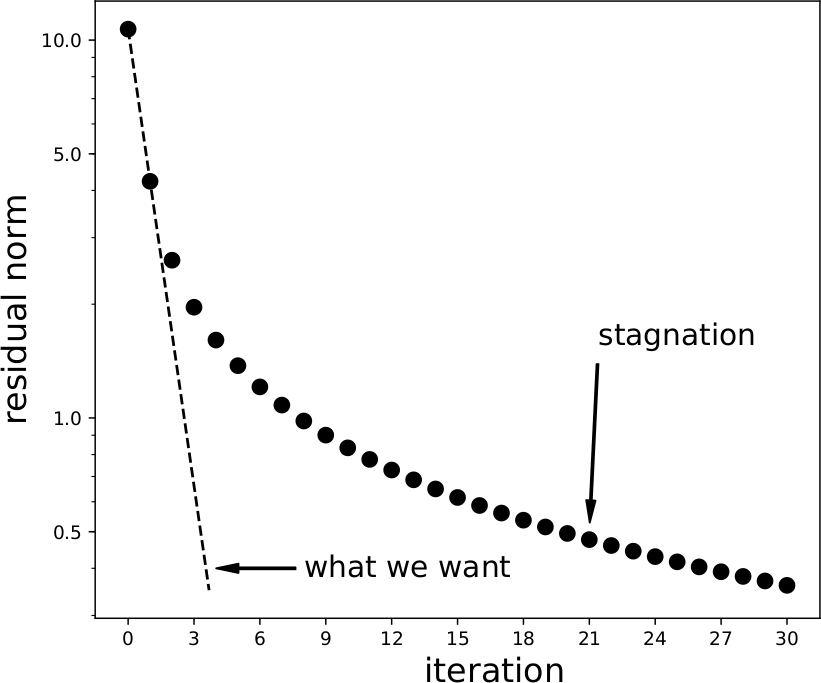
\includegraphics[width=\textwidth]{images/stagnation.png}
\end{column}
\end{columns}

\bigskip
\begin{itemize}
\item<2> Achi Brandt, an inventor of multigrid:
\begin{quotation}
Stalling numerical processes must be wrong.

Whenever the computer grinds very hard for

small or slow effect, there must be a better

way to achieve the same goal.
\end{quotation}

\only<1>{\vspace{14mm}}

\vspace{-19mm}
\hfill \includegraphics<2>[width=0.18\textwidth]{images/abrandt.jpg}
\end{itemize}
\end{frame}


\begin{frame}{Jacobi and Gauss-Seidel iterations \emph{as smoothers}}
\begin{itemize}
\item observation:

functions become

\emph{much smoother}

after a few

iterations

\item the first multigrid

paper (Federenko, 

1961) observed

this?
\end{itemize}

\vspace{-40mm}

\only<1>{
\hfill 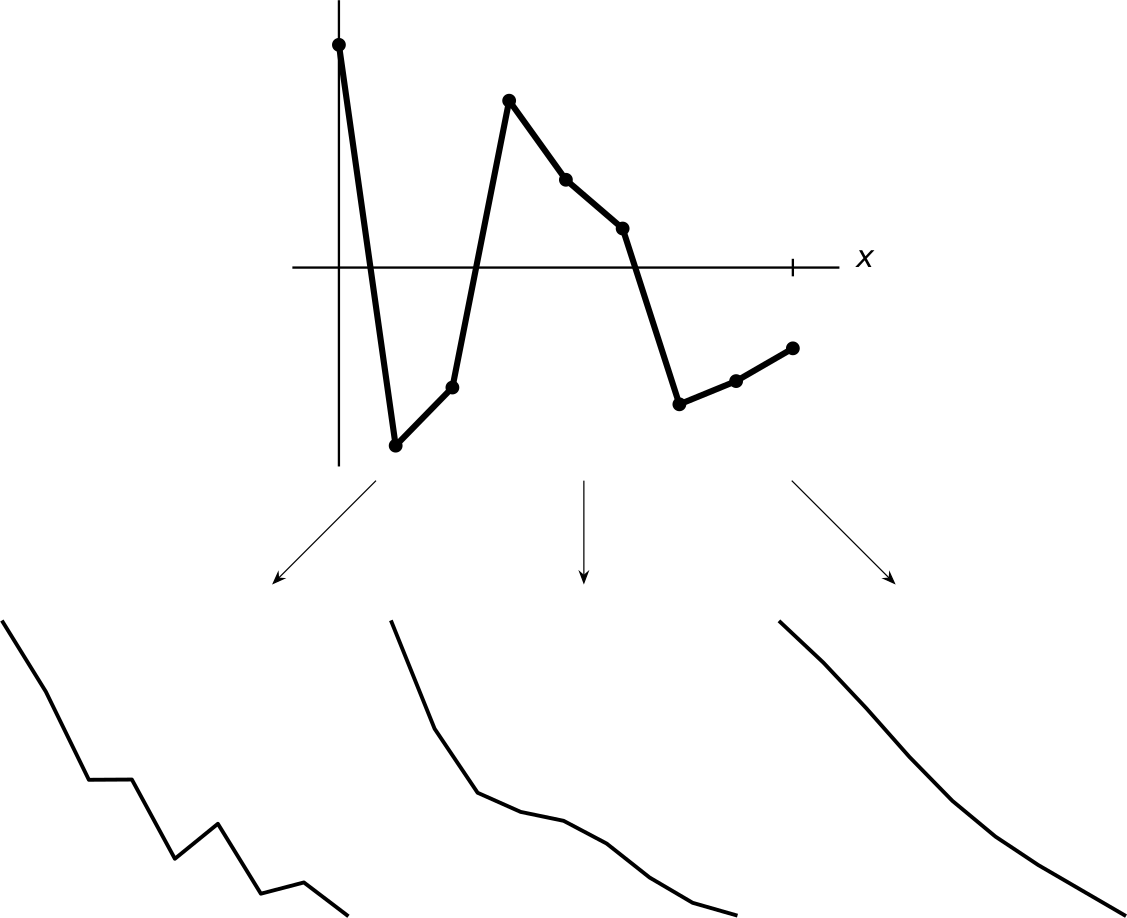
\includegraphics[height=0.75\textheight]{images/smoothing-space.png}

\hfill {\scriptsize Jacobi \hspace{17mm} $\alpha=\frac{2}{3}$ Jacobi \hspace{12mm} Gauss-Seidel \hspace{3mm}}
}
\only<2>{
\hfill 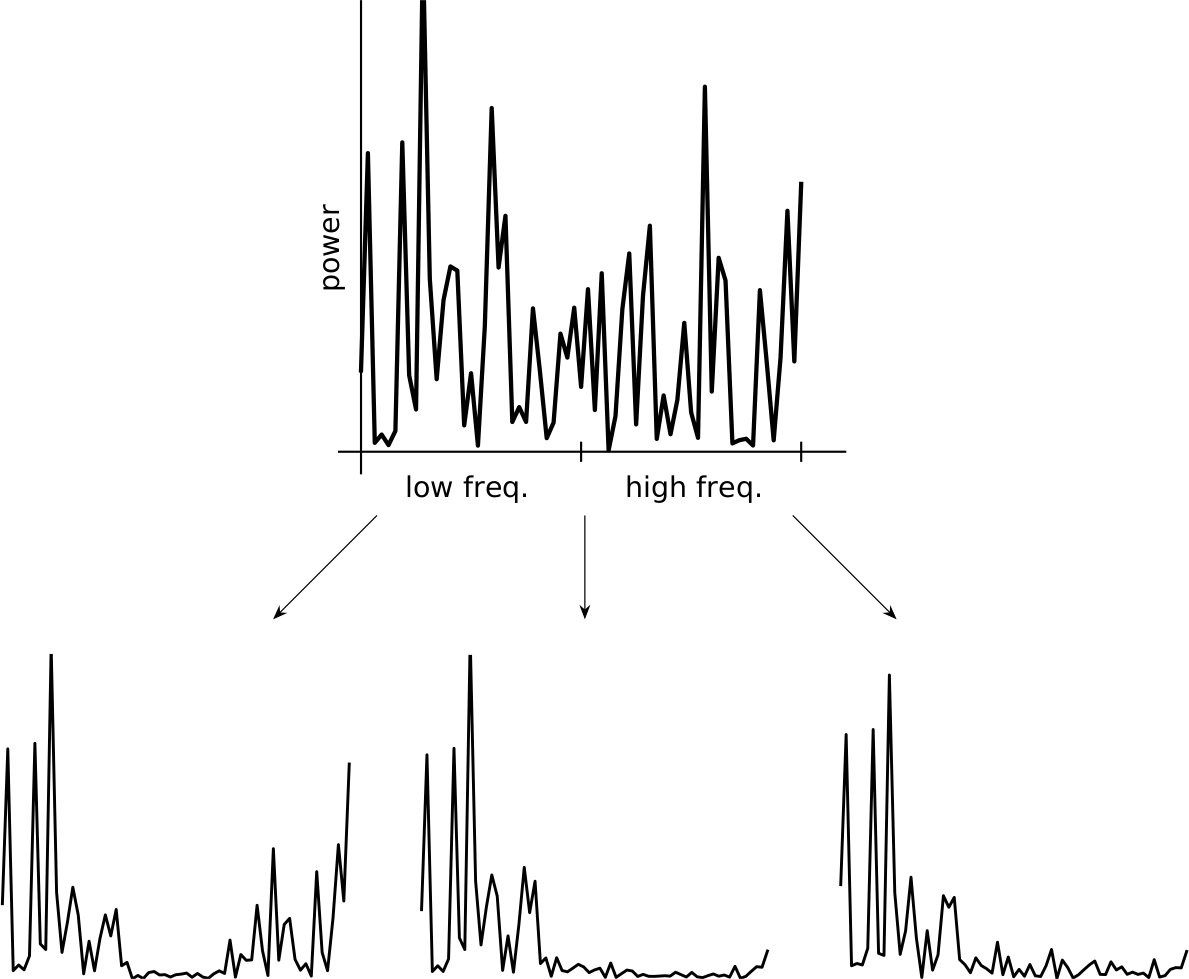
\includegraphics[height=0.75\textheight]{images/smoothing-freq.png}

\hfill {\scriptsize Jacobi \hspace{17mm} $\alpha=\frac{2}{3}$ Jacobi \hspace{12mm} Gauss-Seidel \hspace{3mm}}
}
\end{frame}


\section{2-grid method, and the coarse-grid correction}

\begin{frame}{grid transfers}

\begin{itemize}
\item multiple grid resolutions will allow us to exploit smoothers to generate fast solutions, but we need \emph{grid transfer} operators between the different grids

{\large
$$
\includegraphics[width=0.15\textwidth]{images/fine.png} \qquad
\begin{matrix}
\stackrel{\text{\texttt{restrict}}}{\longrightarrow} \\
\stackrel{\text{\texttt{prolong}}}{\longleftarrow} \\ \phantom{foo} \\ \phantom{foo}
\end{matrix}
\qquad 
\includegraphics[width=0.15\textwidth]{images/coarse.png}$$
}

\vspace{-8mm}
\item for a function $\bv$ defined on a finer grid, define its \emph{restriction} $R\bv$ to a coarser grid to be its value on the coarse grid points (\emph{injection}), or restrict by averaging onto the coarser grid (\emph{full weighting})
\item for a function $\bw$ defined on the coarser grid, define its \emph{prolongation} $P\bw$ to a finer grid by (linear) \emph{interpolation}
\item $R$, $P$ are linear operators
	\begin{itemize}
	\item[$\circ$] $R$, $P$ are rectangular (non-square) matrices
	\item[$\circ$] $R P = I$, or approximately so
	\end{itemize}
\end{itemize}
\end{frame}


\begin{frame}[fragile]
\frametitle{2-grid method}
\begin{itemize}
\item put these ideas together!
\item the \emph{2-grid method} approximately solves the PDE on the finer grid:

\bigskip
\begin{minted}[fontsize=\small,xleftmargin=10mm]{python}
def twogrid(v,pre=2,post=2):
    for k in range(pre):
         v = smooth(A,b,v)
    rc = restrict(b - A*v)
    ec = solve(Ac,rc)          # solve error equation
    v = v + prolong(ec)
    for k in range(post):
         v = smooth(A,b,v)
    return v
\end{minted}

\medskip
\item where
\begin{minted}[fontsize=\small,xleftmargin=10mm]{python}
A,b  = discretize(m,m)         # fine grid
Ac,_ = discretize(m/2,m/2)     # coarse grid
\end{minted}
\item \texttt{smooth()} does one Jacobi or GS iteration
\item \texttt{solve()} might be Gaussian elimination, etc., for \, $A^c \be^c = \br^c$
\end{itemize}
\end{frame}


\begin{frame}{the error equation}
\begin{itemize}
\item what do I mean by the \emph{error equation}?
\item for linear system $A\,\bu=\bb$, consider $\bv$ which is \emph{not} a solution

\begin{definition}
for any vector $\bv$, the \emph{error equation} corresponding to the linear system $A\,\bu = \bb$ is the equation
	$$A\,\be = \br(\bv)$$
\end{definition}

\item here's the logic:
\begin{align*}
    \be &= \bu - \bv                   &&\text{\emph{definition of the error}}\\
    A\, \be &= A \bu - A \bv           &&\text{\emph{multiply by $A$}}\\
    A\, \be &= \bb - A \bv = \br(\bv)  &&\text{\emph{error equation}}
\end{align*}
\end{itemize}
\end{frame}


\begin{frame}[fragile]
\frametitle{the coarse grid correction}
\begin{itemize}
\item the essential 3 lines in \,\texttt{twogrid()} form a \emph{coarse-grid correction}:

\medskip
\begin{minted}[fontsize=\small,xleftmargin=10mm]{python}
rc = restrict(b - A*v)     # restrict the residual
ec = solve(Ac,rc)          # coarse-grid solve
v = v + prolong(ec)        # add back as correction
\end{minted}

\smallskip
\item this is a kind of simple iteration: \qquad $\bv \leftarrow \bv + P (A^c)^{-1} R (\bb - A\bv)$
\item define the \emph{coarse-grid correction matrix}:
	$$B^c = P (A^c)^{-1} R$$
\item so \,\texttt{twogrid()} mixes two flavors of simple iteration:
\begin{align*}
\bv &\leftarrow \bv + M^{-1} (\bb - A\bv) &&\text{\emph{the smoother}} \\
\bv &\leftarrow \bv + B^c (\bb - A\bv) &&\text{\emph{the coarse-grid correction}}
\end{align*}

\medskip
\item the question: is $B^c \approx A^{-1}$?  \only<2>{\hspace{20mm} \alert{yes, for smooth inputs}}
\end{itemize}
\end{frame}


\begin{frame}[fragile]
\frametitle{2-grid method: the effect on error}
\begin{itemize}
\item look at \,\texttt{twogrid()} again:

\medskip
\begin{minted}[fontsize=\small,xleftmargin=10mm]{python}
def twogrid(v,pre=2,post=2):
    for k in range(pre):
         v = smooth(A,b,v)
    rc = restrict(b - A*v)
    ec = solve(Ac,rc)
    v = v + prolong(ec)
    for k in range(post):
         v = smooth(A,b,v)
    return v
\end{minted}

\bigskip
\item a fairly-quick calculation shows that \,\texttt{twogrid()} applies a linear operator which is \alert{close to zero} to the starting error $\be=\bu-\bv$:
	$$\be \leftarrow (I - M^{-1} A)^{\text{\texttt{post}}} (I - B^c A) (I - M^{-1} A)^{\text{\texttt{pre}}} \be$$

\medskip
\item<2> question: how should we solve the coarse-grid problem $A^c \be^c = \br^c$?
\end{itemize}
\end{frame}


\section{V-cycle multigrid}

\begin{frame}{hierarchy of grids}
\begin{itemize}
\item if we can have two levels of grids, we can have many!
\item when faced with a coarse-grid solve, just do another 2-grid \dots and keep going down to some \emph{easy} coarse grid

\bigskip\medskip
\hfill 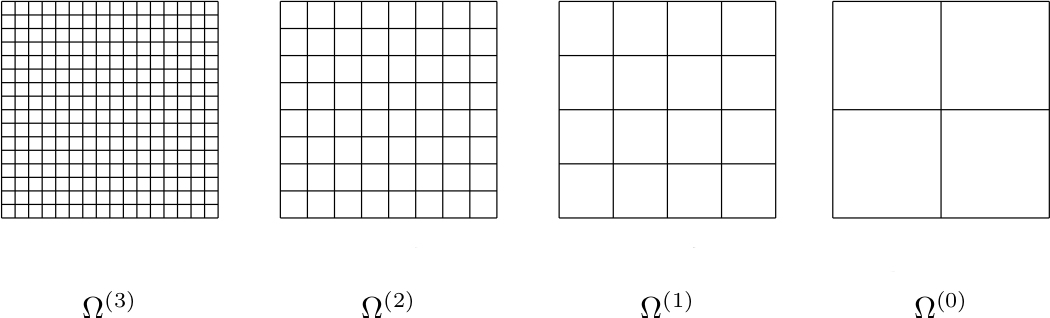
\includegraphics[width=0.8\textwidth]{images/multigrid-grids.png}

\medskip
\item restrictions $R$ and prolongations $P$ are needed in this \emph{grid hierarchy}

\end{itemize}
\end{frame}


\begin{frame}[fragile]
\frametitle{recursive V-cycle}
\begin{minted}[fontsize=\small,xleftmargin=10mm,texcomments]{python}
def vcycle(b,v,lev,pre=2,post=2):
    A,_ = discretize(lev)
    if lev == 0:
        return solve(A,b)    # the buck stops here
    for k in range(pre):
         v = smooth(A,b,v)
    rc = restrict(b - A*v)
    ec = vcycle(r,0,lev-1)   # descend a grid level
    v = v + prolong(ec)
    for k in range(post):
         v = smooth(A,b,v)
    return v
\end{minted}

\vspace{-5mm}
\hfill 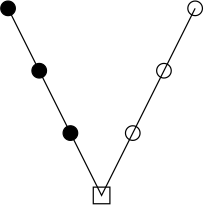
\includegraphics[width=0.15\textwidth]{images/vcycle.png}

\vspace{-8mm}
\hspace{5mm} 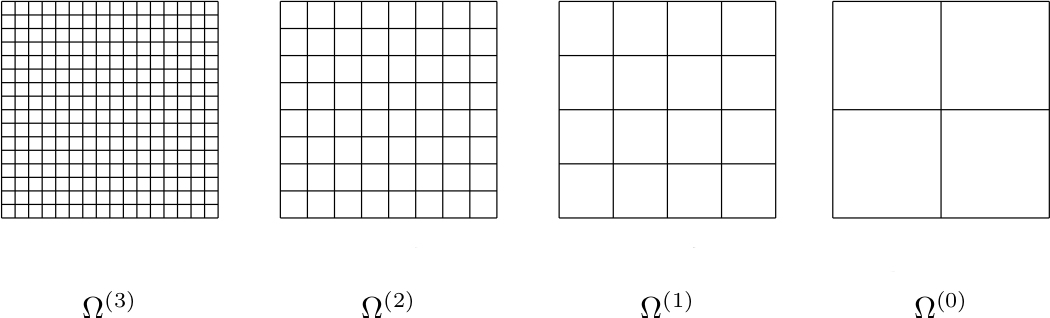
\includegraphics[width=0.6\textwidth]{images/multigrid-grids.png}
\end{frame}


\section{multigrid as an optimal solver}

\begin{frame}{how well does it work?}
\begin{itemize}
\item so, how well does it work on our Poisson problem

\,$-\grad^2 u=f$?

\vspace{-5mm}
\hfill 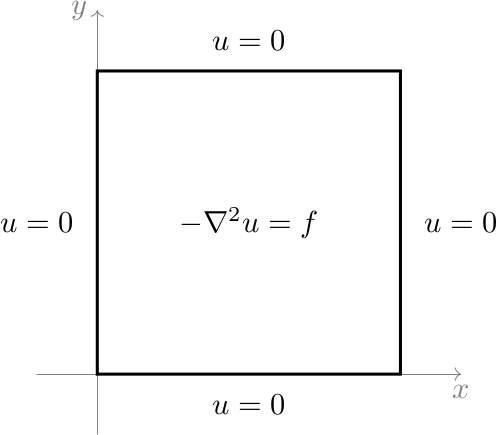
\includegraphics[width=0.2\textwidth]{images/poisson.png}

\vspace{-13mm}
\item absurdly well!
\item here is scaling out to $m=4097$, when $N=1.6\times 10^7$
\end{itemize}

\medskip
\begin{center}
\only<1>{ % Figure 7.2
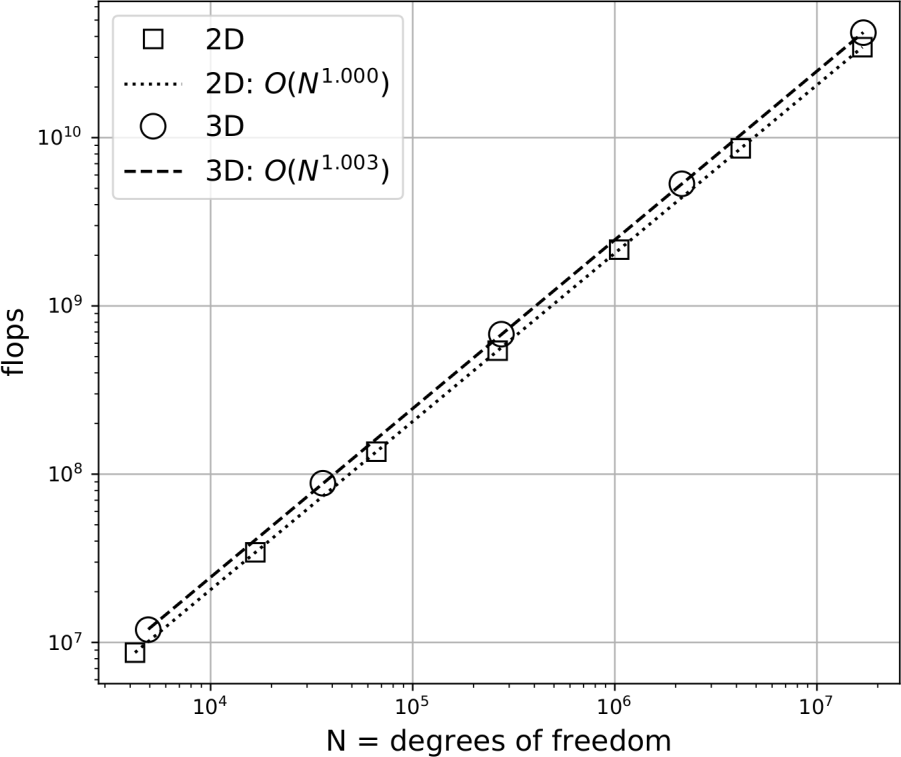
\includegraphics[height=0.6\textheight]{images/poisson-optimal-flops.png} \hspace{10mm}
}
\only<2>{ % Figure 7.4
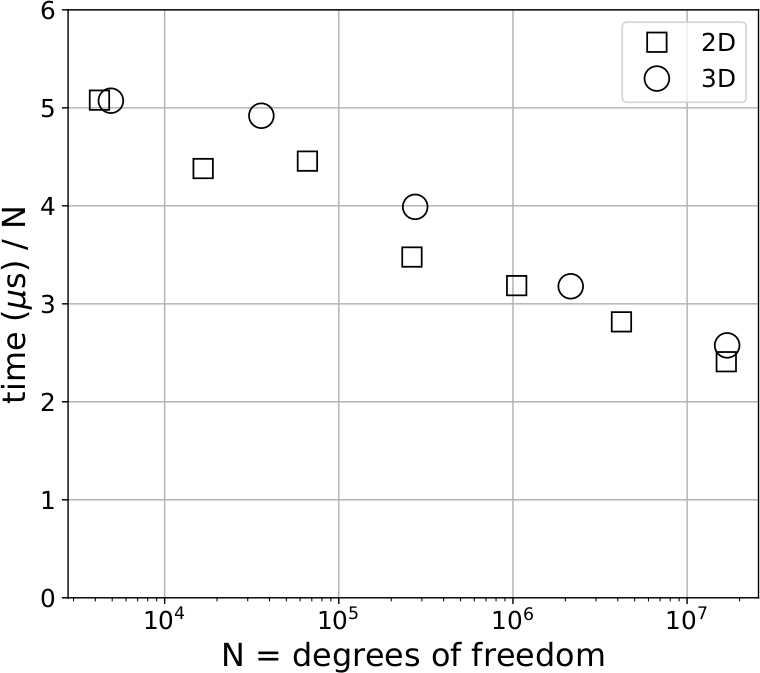
\includegraphics[height=0.6\textheight]{images/poisson-optimal-timeperdof.png} \hspace{10mm}
}
\end{center}
\end{frame}


\begin{frame}{on multigrid costs: single V-cycle}
\begin{itemize}
\item let us analyze the work (flops) of applying a single V-cycle
    \begin{itemize}
    \item[$\circ$] note: multiple V-cycles are generally needed to solve the problem
    \end{itemize}

\medskip
\begin{definitions}

\vspace{-4mm}
\begin{align*}
|\Omega^{(k)}| &= (\text{number of grid points (unknowns) on grid $\Omega^{(k)}$}) \\
W_k^{k-1} &= \left(\begin{matrix} \text{smoother work done on grid $\Omega^{(k)}$, plus cost of} \\ \text{restriction \& prolongation to next-coarser grid $\Omega^{(k-1)}$} \end{matrix}\right) \\
W_0 &= (\text{solver work done on the coarsest level})
\end{align*}
\end{definitions}

\medskip
\item $K=3$ case:
\end{itemize}

\vspace{-3mm}
\hfill 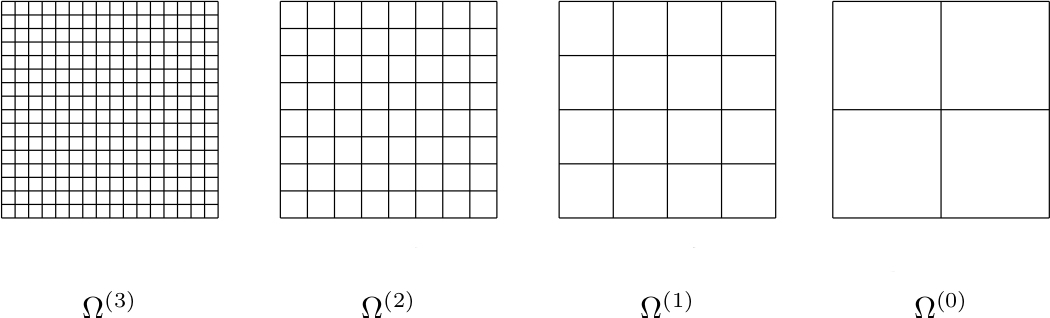
\includegraphics[width=0.65\textwidth]{images/multigrid-grids.png}
\end{frame}


\begin{frame}{on multigrid costs: single V-cycle}
\begin{itemize}
\item total cost of a single V-cycle:
    $$\overline{W} = W_K^{K-1} + W_{K-1}^{K-2} + \dots + W_1^0 + W_0$$
\item for 2D grids, each coarse grid is 4 times smaller:
    $$|\Omega^{(k-1)}| = \tfrac{1}{4} |\Omega^{(k)}|$$

\vspace{-28mm}
\hfill 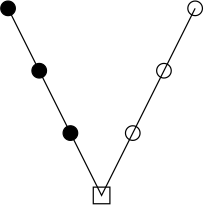
\includegraphics[width=0.13\textwidth]{images/vcycle.png}

\vspace{9mm}
\item since smoothers and restriction/prolongation are $O(1)$ per grid point:
    $$W_k^{k-1} = C |\Omega^{(k)}|$$

    \begin{itemize}
    \item[$\circ$] for some $C$ independent of $k$
    \end{itemize}
\item<2> since $N=|\Omega^{(K)}|$ is the number of points in the finest grid,
\begin{align*}
\overline{W} &= C |\Omega^{(K)}| + C |\Omega^{(K-1)}| + \dots + C |\Omega^{(1)}| + W_0 \\
    &= C N \left(1 + \tfrac{1}{4} + \dots + \tfrac{1}{4^{K-1}}\right) + W_0 \\
    &\approx C N \tfrac{1}{1-(1/4)} = \tfrac{4}{3} C N \hspace{20mm} \text{\alert{optimal}}
\end{align*}
\end{itemize}
\end{frame}


\begin{frame}{multigrid variations}
\begin{itemize}
\item there are many variations on multigrid:
	\begin{itemize}
	\item[$\circ$] choose different smoothers ({\large $\bullet$} is pre-smoother, {\large $\circ$} is post-smoother)
	\item[$\circ$] choose different values for \texttt{pre} and \texttt{post} smoother iterations
	\item[$\circ$] choose different coarse-grid solvers ($\square$)
	\item[$\circ$] repeat the coarse-grid correction a couple of times (\emph{W cycles})
	\end{itemize}

\bigskip\bigskip
\hfill 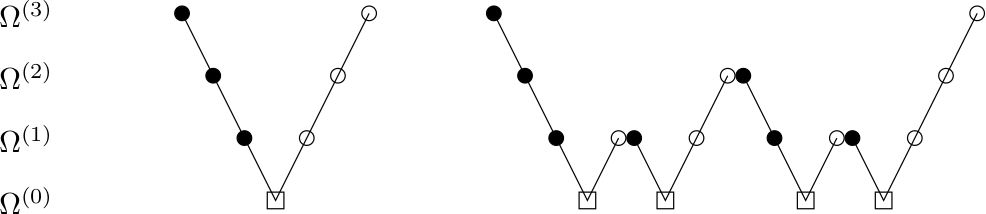
\includegraphics[width=0.8\textwidth]{images/multigrid-cycles.png}
\end{itemize}
\end{frame}


\begin{frame}{summary so far}
\begin{itemize}
\item multigrid combines three conceptual threads:
\begin{enumerate}
\item a few classical iterations, such as Jacobi and GS, are \textbf{cheap smoothers} of the error
\item a \textbf{coarse-grid correction} does a good job of approximating the fine-grid solution when acting on a smooth residual
\item the coarse-grid correction is cheap because \textbf{restriction and prolongation are cheap}
\end{enumerate}

\bigskip
\item<2> but \dots the Poisson problem is too easy
\end{itemize}
\end{frame}


\begin{frame}{minimal surfaces, a nonlinear problem}
\begin{itemize}
\item recall \dots

\vspace{-10mm}
\hfill 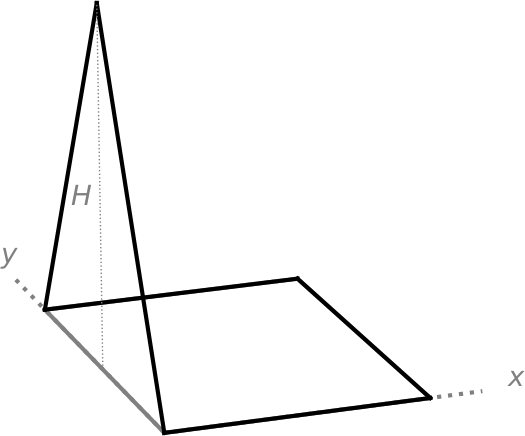
\includegraphics[width=0.25\textwidth]{images/tent.png} 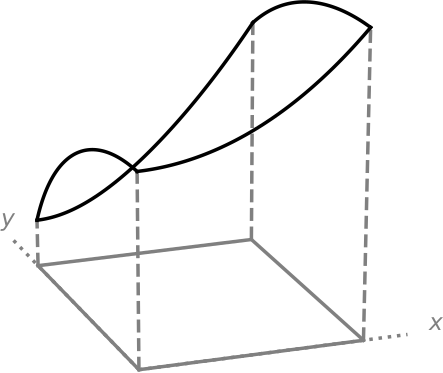
\includegraphics[width=0.25\textwidth]{images/catenary.png}
\end{itemize}

\bigskip
\begin{block}{minimal surface problem} for given boundary function (wire frame) $g(x,y)$, find $u(x,y)$ so that
    $$-\Div \left(\frac{\grad u}{\sqrt{1 + |\grad u|^2}}\right) = 0 \, \text{ on } \Omega, \qquad u\big|_{\partial \Omega} = g$$
\end{block}
\end{frame}


\begin{frame}{discretization gets you \dots harder equations}
\begin{itemize}
\item x
\end{itemize}
\end{frame}


\begin{frame}{details: 9-point stencil with staggered diffusivity}
\begin{itemize}
\item how do you discretize $\ds -\Div \left(\frac{\grad u}{\sqrt{1 + |\grad u|^2}}\right)$?
\item generalize for clarity: \,$\ds -\Div \left(D(w) \grad u\right)$

where
    $$D(w) = (1+w)^{-1/2} \hspace{40mm}$$

\vspace{-24mm}
\hfill 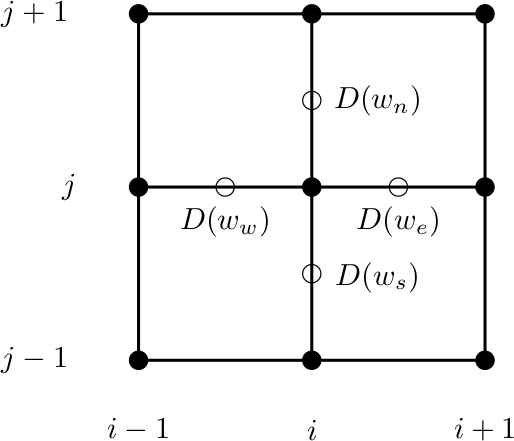
\includegraphics[width=0.3\textwidth]{images/msboxstencil.png}

\vspace{-5mm}
\item then do centered finite-differences using

\emph{staggered} values of $D(w)$ for $w=|\grad u|^2$:
\begin{align*}
-\Div \left(D(w) \grad u\right) &\approx FIXME \\
w_e = \left[|\grad u|^2\right]_{i+1/2,j} &\approx 
\end{align*}
\end{itemize}
\end{frame}


\begin{frame}{Newton's method}
\begin{itemize}
\item x
\end{itemize}
\end{frame}


\begin{frame}{x}
\begin{itemize}
\item x
\end{itemize}

\hfill 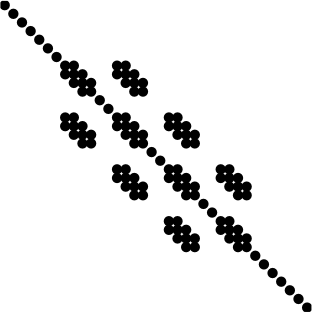
\includegraphics[width=0.3\textwidth]{images/minimal-spy.png}
\end{frame}


\begin{frame}{nonlinear F-cycle solvers}
\begin{itemize}
\item x
\end{itemize}

\hfill 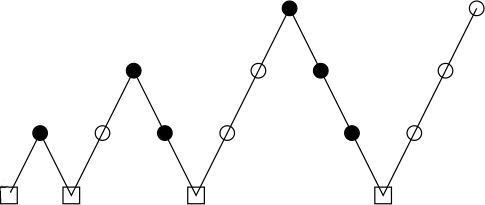
\includegraphics[width=0.3\textwidth]{images/multigrid-fullcycle.png}
\end{frame}


\begin{frame}{minimal surface results}
\begin{itemize}
\item x
\end{itemize}

\hfill 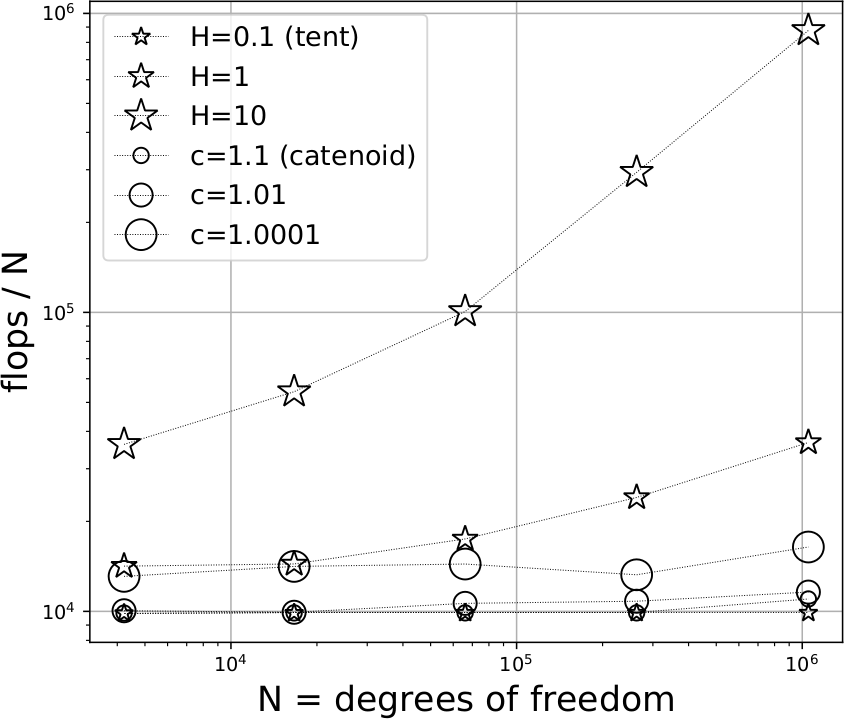
\includegraphics[width=0.3\textwidth]{images/minimal-flopsperdof.png}

FIXME: do demo
\end{frame}


\begin{frame}{references}

\setbeamerfont*{itemize/enumerate body}{size=\footnotesize}
\setbeamerfont*{itemize/enumerate subbody}{parent=itemize/enumerate body}

\begin{columns}
\begin{column}{0.8\textwidth}
\begin{itemize}
\item[] \textbf{A.~Brandt (1977)}. \emph{Multi-level adaptive solutions to boundary-value problems}, Mathematics of Computation 31 (138), 333--390
    \begin{itemize}
    \item[$\circ$] the guru of multigrid
    \end{itemize}
\item[] \textbf{W.~Briggs, V.~E.~Henson, \& S.~McCormick (2000)}.  \emph{A Multigrid Tutorial}, 2nd ed., SIAM Press, Philadelphia
    \begin{itemize}
    \item[$\circ$] straightforward introduction
    \end{itemize}
\item[] \textbf{E.~Bueler (2021)}. \emph{PETSc for Partial Differential Equations}, SIAM Press, Philadelphia
    \begin{itemize}
    \item[$\circ$] preconditioners, many multigrid examples
    \end{itemize}
\item[] \textbf{H.~Elman, D.~Silvester, \& A.~Wathen (2014)}. \emph{Finite Elements and Fast Iterative Solvers: With Applications to Incompressible Fluid Dynamics}, 2nd ed., Oxford U.~Press
    \begin{itemize}
    \item[$\circ$] multigrid in FE and fluids contexts
    \end{itemize}
\item[] \textbf{R.~Fedorenko (1961)}.  \emph{A relaxation method for solving elliptic difference equations}, USSR Comput.~Math.~Math.~Phys.~1, 922--927
    \begin{itemize}
    \item[$\circ$] the first multigrid paper
    \end{itemize}
\item[] \textbf{U.~Trottenberg, C.~Oosterlee, \& A. Schuller (2001)}.  \emph{Multigrid}, Elsevier
    \begin{itemize}
    \item[$\circ$] a comprehensive view
    \end{itemize}
\end{itemize}
\end{column}
\begin{column}{0.17\textwidth}
\hfill 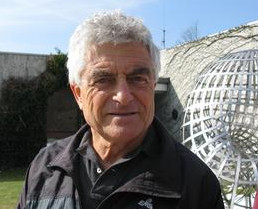
\includegraphics[width=\textwidth]{images/abrandt.jpg}

\hfill {\scriptsize \emph{Achi Brandt}}

\vspace{7mm}
\hfill 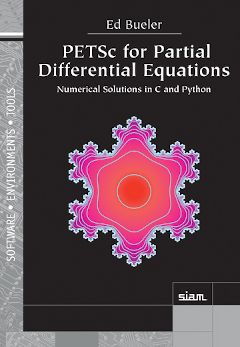
\includegraphics[width=0.9\textwidth]{images/bueler.jpg}

\vspace{20mm}
\end{column}
\end{columns}
\end{frame}

\end{document}
